\documentclass[ARTICLETHERMIC.tex]{subfiles}

\begin{document}

The algorithm described in this paper is based on the implementation of the classical MLR (Multiple Linear Regression) method presented in \cite{eischeid_creating_2000}. The MLR method is robust and well known and can indirectly account for local effects, such as topography, land cover, land use and surface water. While creating serially complete daily datasets of air temperature and total precipitation for the western U.S., \cite{eischeid_creating_2000} found that the MLR method consistently outperformed the other classical methods tested (normal ratio, inverse distance, optimal interpolation, and single best estimator). The same result was also found by \cite{xia_forest_1999} for a study in Bavaria, Germany. Moreover, in a study conducted in Iran for different climate conditions (dry to extra humid conditions), \cite{kashani_evaluation_2011} found that the estimation obtained with the MLR method compared well with those obtained with more recent methods, more specifically the artificial neural network (reference) and the genetic programming (references) techniques.

\Cref{fig:fillworker_flowchart} presents a flowchart of the algorithm used in WHAT for filling the gaps in the daily weather dataset for a given target station using data from the neighboring stations. The algorithm consists of two nested loops: the external `Loop A' iterates over the weather variables in the dataset of the target station (min, max, and mean air temperature and total precipitation), while the inner `Loop B' iterates over the missing values in the data series for a given variable. Each missing value is estimated independently with a two-step procedure. The first step of the procedure consists in the selection of the neighboring stations. The second step consists in building a MLR model and estimating the missing value in the dataset of the target station. 

\begin{figure}[!p]
    \centering
    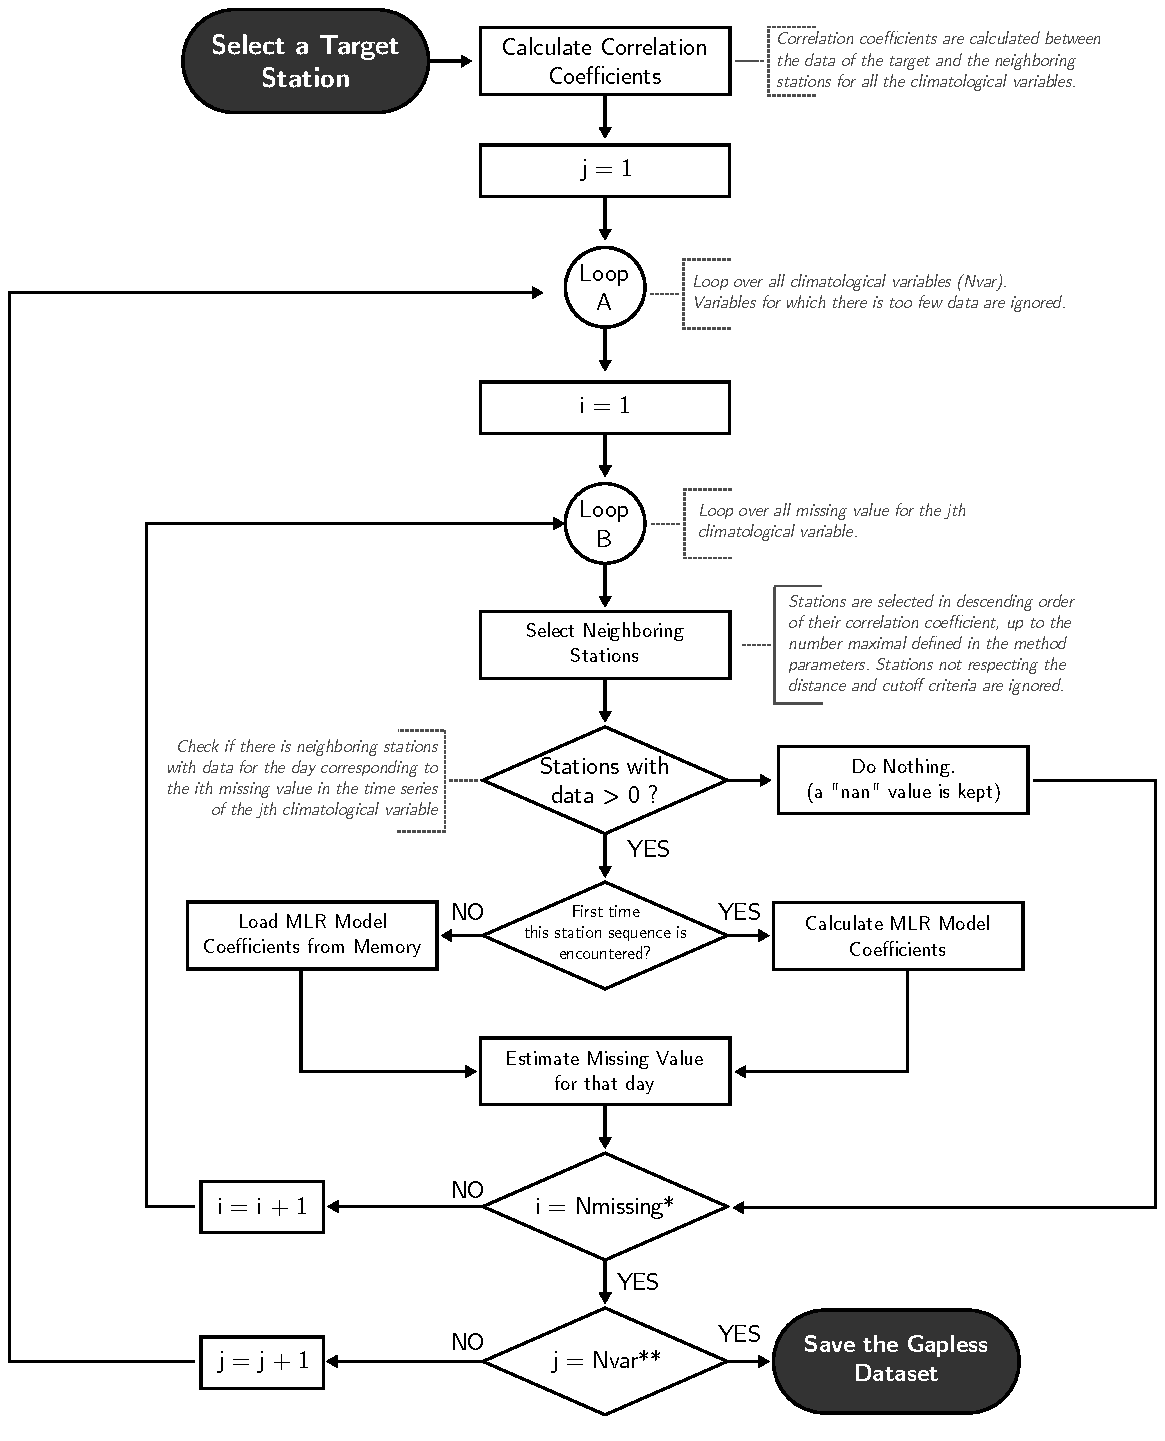
\includegraphics[width=\textwidth]{img/Flowchart-filling_missing_weather.pdf} 
    \caption{}
    \label{fig:fillworker_flowchart}
\end{figure}

\subsection{Loop A}

\subsubsection{Quality Control}

Prior to the analysis of weather time series, it is important to apply quality control constraints to ensure that the data do not violate obvious constraints associated with minimum, maximum, and average daily air temperature and daily cumulative precipitation. 

The program will identify irregularities or inconsistencies to insure that maximum, minimum and average daily temperatures are coherent for a given day and that all daily precipitation values are positive. Erroneous values are replaced by nan values in the dataset. These values will subsequently be estimated by the program from neighboring stations.

\subsubsection{Station Correlation Assessment}

The first step consists in calculating the correlation coefficients between data of the target station and those of the neighboring stations for each of the four weather variables: minimum, maximum and average daily temperatures and daily cumulative precipitation. These coefficients are calculated for the entire time-series for each neighboring station individually. If there are less than 182 synchronous values between the data of the target station and those of a neighboring station for a given variable, the correlation is not computed and a ‘‘NaN’’ value is kept instead.

\subsection{Loop B}

\subsubsection{Selection of the neighboring stations}
%Problems arise when
%using climatological data because of missing values and
%the varying availability of stations through time

%The number (never greater than four) of neighboring
%stations meeting the criteria is not fixed in time. It varies
%depending on available station data for the year/month/
%day in question. As such, the interpolation models may
%also change in time.

The selection of surrounding stations is critically important for the accurate estimation of missing weather data (Eischeid et al., 1995). Problems arise though because of synchronized missing values in the target and neighboring weather station datasets that varies trough time. This is illustrated in Table 8.1, where theoretical time-series of air temperature data with a realistic distribution of missing values are presented.

In \cref{tab:selectStations}, there are missing values in the target station dataset for days 2, 4, and 5. The missing value on day 2 will then be estimated with the data of the neighboring stations Y1, Y3, and Y4 since station Y2 is also missing a value on this day. All neighboring stations will be used for the estimation of the missing value on day 4, while only stations Y1 and Y2 have data available for the estimation of the missing value on day 5.

Data correlation between two stations will generally decreases as the horizontal and vertical distances increase. It is possible to specify a cutoff distance and a cutoff altitude difference for which neighboring stations that fall above these cutoff values are ignored by the program. The default values are set to 100 km and 350 m for the horizontal and vertical distance respectively based on the literature (Simolo et al., 2010; Tronci et al., 1986; Xia et al., 1999).

\begin{table}[!hb]
\newcommand{\nan}{\multicolumn{1}{c}{\textbf{nan}}}
\center
\caption{This table shows some data}
\begin{tabular}{
S[table-format = 1]
*5S[table-format = 2.1]
}
\toprule
& {Target} & \multicolumn{4}{c}{Neighbors} \\
\cmidrule(lr){3-6}
{Day} & {Y} & {X1} & {X2} & {X3} & {X4} \\
\midrule
%\rowcolor{gray!30}
1 & 11.0 & 12.0 & 12.0 & 12.5 & 10.0 \\
2 & \nan & 12.0 & \nan & 13.0 & 12.2 \\
3 &  7.5 &  8.5 &  8.5 &  8.0 &  8.9 \\
4 & \nan &  6.0 &  4.5 &  5.0 &  4.4 \\
5 & \nan &  8.0 &  8.5 & \nan & \nan \\
\bottomrule
\end{tabular}
\label{tab:selectStations}
\end{table}

Since the number of neighboring stations with available data is not fixed in time, it is not possible to use a single MLR model to fill all the missing values for the target station all at once. For each missing value in the target station dataset, the program keeps only the datasets of the neighboring stations that also have data at this particular time. Data series of stations that do not respect the cutoff criteria for distance and elevation differences are also ignored. Data from neighboring stations are selected in descending order of their correlation coefficient with the target station, up to a maximal number of stations defined in the method parameters. The default value for the maximal number of neighboring station was set to four, based on the literature (Eischeid et al., 1995; Xia et al., 1999).

If for a given day, no neighboring stations have a measured value to fill a gap in the target station dataset, no calculation is done and a ‘‘NaN’’ value is kept in the series instead and the program pass to the next missing value in the target series.

\subsubsection{Multiple Linear Regression Model}
First, the program will be checking if the sequence of neighboring stations has already been encountered for the current weather variable and, if so, will load the MLR parameters from memory and will directly estimate the missing value. Otherwise, the model will generate a new MLR model using either an Ordinary Least Square (OLS) or a Least Absolute Deviations (LAD) criteria (both options are available). Since daily precipitation series generally represented by long-tailed, positively skewed, distributions, the LAD criterion is typically a better option than the OLS criteria for handling this kind of distribution because it is more robust to outliers (Eischeid et al., 2000, 1995). The downside is an increase in computation time. The MLR using a LAD criterion is computed in WHAT with an iterative reweighted least-squares method (Schlossmacher, 1973; (Eischeid et al., 1995).


\subsubsection{Estimating Missing Daily Values}

Once the parameters of the MLR model for a given day with a missing value are known, the missing value in the target time series is estimated as:

\begin{equation}
    X(t) = a_0 + \sum_{i=1}^{N} a_i \cdot Y_i(t)
\end{equation}

where Y(t) is the missing value of the target station estimated at time t, Xi are the synchronous values of the neighboring stations, ai are the regression coefficients and N is the total number of neighboring stations used for the regression, up to the maximal value defined in the method (default is four).

When all missing values in the target station dataset have been estimated, the resulting gapless time series is saved in a ‘‘.out’’ file. Detailed information about the estimated values are saved in an accompanying ‘‘.log’’ file (see Section 8.3.1).

\subsection{Step 3: Validation}

WHAT also includes an option to perform a validation of the method used for a particular weather dataset with a jackknife procedure. This option is an advanced feature that can be activated by changing the value of the field ‘‘Full Error Analysis’’ from 0 to 1 in the file named ‘‘WHAT.pref’’ (see Section 8.3.1).

More specifically, when this option is activated, WHAT will estimate a value for the target station for every day of the time series. In other words, loop B in the flowchart of Figure 8.1 will run over all the days of the dataset and not only over days for which there is a missing data. In addition, the memory feature will be deactivated and a MLR model will be estimated for each day independently. If a measured value is present for the current day being estimated, this value will be temporarily discarded from the data series to avoid self-influence of the observation on the estimation procedure

Consequently, the activation of this feature will significantly raise the computation time for filling the gaps in weather time series and should be used only when a detailed analysis of the estimation errors is required. The default information provided in the ‘‘.log’’ should contain sufficient material to fill the needs of a large number of projects. Thus, this process leads to the production of a weather time-series for which every value has been estimated in WHAT. The results are saved in a tsv (tab-separated values) text file with the extension ‘‘.err’’ that is named after the station name and ID similarly to the ‘‘.log’’ and ‘‘.out’’ files.
The accuracy of the estimation technique can then be assessed by comparing the estimated weather data with the respective non-missing observations in the original weather data file. There is currently no tool provided in WHAT to directly analyze the results from the Jackknife procedure. However, all the source code that has been written? for the production of the figures of Section 8.4 can be downloaded freely on GitHub at (https://github.com/jnsebgosselin/WHAT).

\end{document}

%The first step of the procedure consists in the selection of the neighboring stations, whose data will be used to estimate the missing value in the dataset of the target station. The second step consists in building a MLR model and estimating the missing value.

%Among these techniques, methods based on the use of data from neighboring stations are generally favored to within-station methods, i.e. those that only use data from the series being filled.

%have been proven to perform poorly compared to methods based on the use of data from neighboring stations for the reconstruction of daily precipitation time series (Eischeid et al., 1995; Kemp et al., 1983; Simolo et al., 2010).

%The creation of a serially complete weather dataset generally consists in the replacement of missing daily data with estimated values calculated from simultaneous observations at nearby stations. 

%Numerous spatial interpolation techniques exist for handling the missing data in the weather time series of a given station by using data from irregularly spaced neighboring station (e.g. simple arithmetic averaging, inverse distance method, single best estimator and multiple regression analysis).
